\documentclass[12pt,a4paper]{article}
\usepackage{styles/preamble}

% =================================================
% НАЧАЛО ДОКУМЕНТА
% =================================================

\begin{document}

\import{titlepage/}{title_old} % Титульный лист
\import{titlepage/}{title_new} % Титульный лист

\tableofcontents % Так выглядит вставка с содержанием


\section{Самая главная секция}

На первых двух страницах приведены два варианта титульника: старый и новый. Далее приведён возможный вариант стил


\subsection{Шрифт}

В качестве шрифтов используются \href{https://fonts.google.com/specimen/Raleway}{Raleway} и \href{https://fonts.google.com/specimen/Anonymous+Pro}{AnonymousPro}.

\begin{multicols}{2}
	\begin{itemize}
		\item Raleway, regular.
		\item \textit{Raleway, italic.}
		\item \textbf{Raleway, bold.}
		\item \textbf{\textit{Raleway, bold italic.}}
		\item \texttt{AnonymousPro, mono.}
		\item \textit{\texttt{AnonymousPro, mono italic.}}
		\item \textbf{\texttt{AnonymousPro, mono bold.}}
		\item \textbf{\texttt{AnonymousPro, mono bold italic.}}
	\end{itemize}
\end{multicols}


\subsection{Математические формулы}

\marginpar{\textcolor{olive}{\textbf{TODO} МБ есть формула поинтереснее?}}

В качестве примера приведена формула интегрирования по частям для определённого интеграла \eqref{simple_equation}.

\begin{equation} \label{simple_equation}
\INT_a^b u dv = uv \Big|_a^b - \INT_a^b v du
\end{equation} 


\subsection{Листинг}

В качестве примера приведена простая программа на языке Python (Листинг~\ref{lst:simple_code}). 

\lst{python}{code/main.py} 
\captionof{listing}{Простая программа на Python}
\label{lst:simple_code}

% Принудительно делаем новую страницу для красоты.
% Вообще, так делать не стоит, т.к. если вдруг что-то поменяете сверху,
% то может смотреться некрасиво
\newpage


\subsection{Картинка}

Можно вставлять картинки. Я так и сделал (Рис.~\ref{pic:luthadel}).
\begin{figure}[!h]
	\centering
	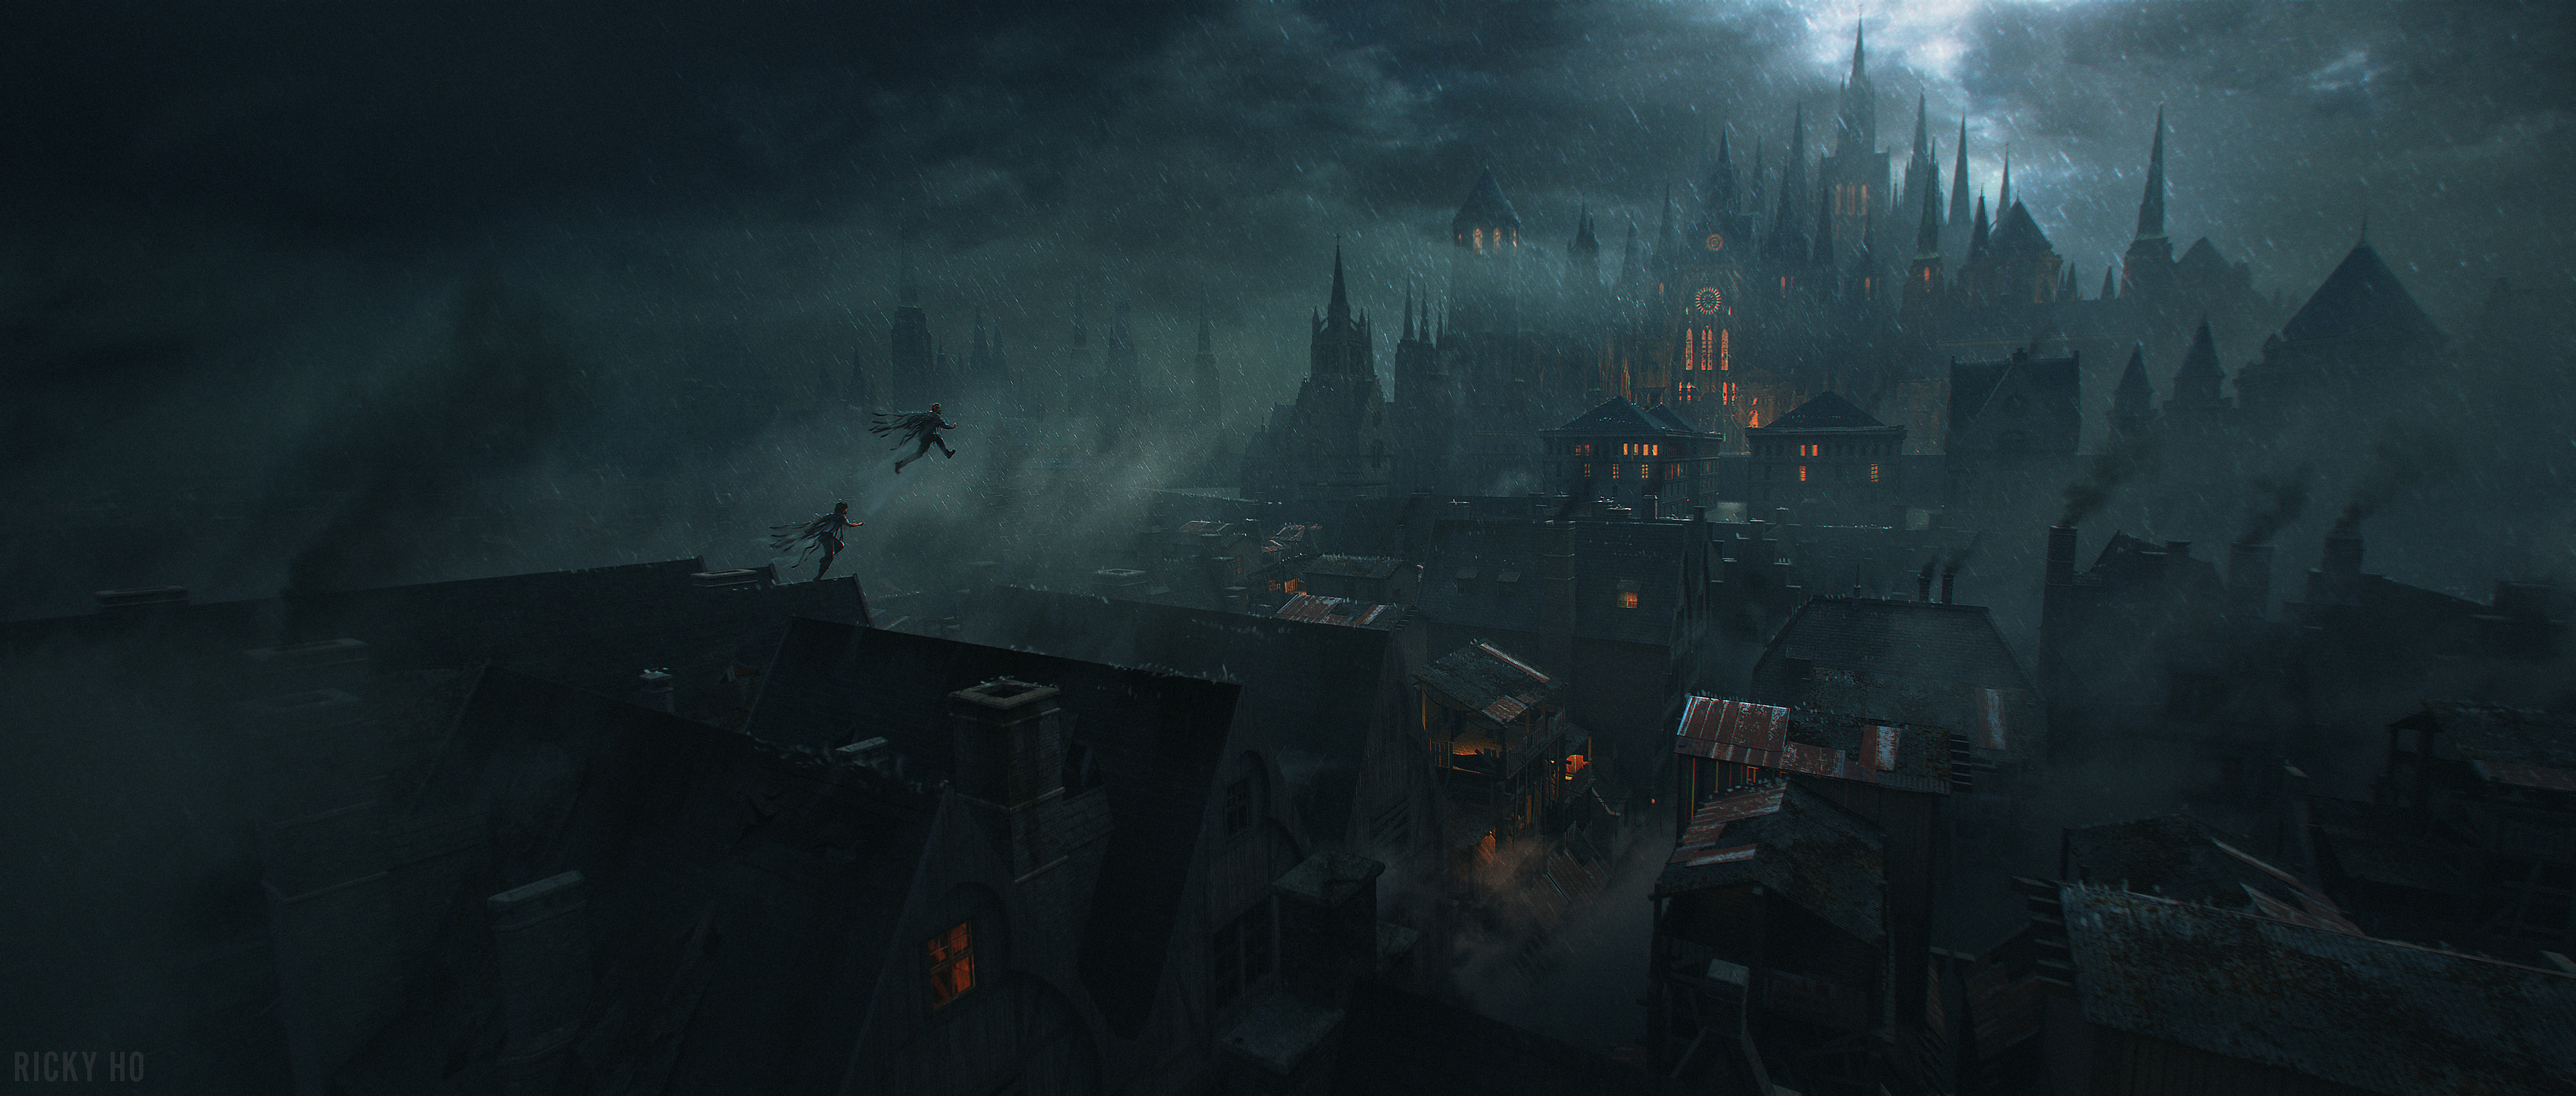
\includegraphics[width=1.0\textwidth]{pic/ricky-ho-mistborn-luthadel-city-rickyho}
	\caption{Mistborn: Luthadel at night by Ricky Ho}
	\label{pic:luthadel}
\end{figure}


\subsection{Красивая нумерация}

Можно красиво нумировать списки:

\begin{enumerate}[(a)]
    \item Вот раз.
    \item А вот два, причём:
    \begin{enumerate}[1 $\to$]
    	\item Можно использовать любые символы для нумерации.
    	\item Даже математические!
    \end{enumerate}
\end{enumerate}


\subsection*{Секция, которая не отобрзится в содержании и без цифры!}

\textcolor{gray}{\xout{этого текста нет на картах!}}


\subsection{Таблички}

Таблицы можно делать с помощью пакета \texttt{csvsimple}\footnote{Для несложных таблиц.} или \texttt{pgfplotstable}\footnote{Для таблиц с большим количеством разнородной информации.}. А можно вставлять напрямую:

\begin{table}[h!]
	\centering
	\begin{tabular}{|c|l|l|} \hline
		& \textbf{Имя} & \textbf{Фамилия} \\ \hline
		1 & Гаррье & Дюбуа \\ \hline
		2 & Ким & Кицураги \\ \hline
	\end{tabular}
	\caption{Главные герои Disco Elysium.}
	\label{table:disco_main_characters}
\end{table}

\end{document}